% !TeX program = xelatex
% !TeX encoding = utf8
% !TeX root = Fading.tex
% vim: set ts=2 sw=2 noet:

\documentclass[
	% show when a line is too long (drafting)
	overfullrule,
	% page size and margins
	paper = a4, twoside, openright, BCOR = 5mm,
	headinclude, footexclude,
	% font size
	fontsize = 11pt,
	% style of empty pages (after chapters)
	cleardoublepage = empty,
	% extra sections
	titlepage, abstract = on,
	% header and footers
	automark,
]{scrreprt}

%% Language configuration
\usepackage{polyglossia}
\setmainlanguage{english}

% Use a different font for german
\usepackage{xcolor}
\setotherlanguage{german}
\newfontfamily{\germanfont}{Roboto Condensed Light}

%% Custom packages
\usepackage{tex/docmacros}
\usepackage[draft]{tex/docstyle}

%% Pretty figures
\usepackage{circuitikz}  % Electric diagrams
\usepackage{pgfplots}    % Pretty plots
\usepackage{tikz}        % Pretty drawings
\usepackage{tikz-3dplot} % More dimensions!

\pgfplotsset{compat=newest}
\usetikzlibrary{
	external,
	calc,
	positioning,
	backgrounds,
	decorations.pathreplacing,
	calligraphy,
	decorations.markings,
	matrix,
	arrows,
	patterns,
}
% \tikzexternalize[
% mode=graphics if exists,
% figure list=true]
\pgfdeclarelayer{background}
\pgfdeclarelayer{foreground}
\pgfsetlayers{background,main,foreground}

\usepackage{graphicx}   % Include pictures
\usepackage{subcaption} % Subfigures

%% Placeholders
\usepackage{skeldoc}

%% Nicer tables
\usepackage{tabularx}
\usepackage{booktabs}

%% Writing units
\usepackage{siunitx}
% this one is for siunitx v3, debian and older systems
% still have only siunitx v2 installed
% \sisetup{uncertainty-mode = separate}
\sisetup{separate-uncertainty}

%% Load bibliography 
\addbibresource{Fading.bib}

%% Recompute page margins
\KOMAoptions{DIV=default}

%% Metadata
\title{Multipath fading demonstration using software defined radio}
\author{Naoki Sean Pross \and Sara Cinzia Halter}
\date{Fall semester 2021}

\begin{document}

	\hypersetup{pageanchor = false}

	%% TODO: create a proper titlepage
	\maketitle
	% % vim: set ts=2 sw=2 noet:

\begin{titlepage}
	\newgeometry{
		outer = 3cm, inner = 3cm,
	}
	\centering

	{\huge\bfseries\sffamily
		Multipath Fading Demonstration Platform using Software Defined Radio
	\par}

	\vspace{1cm}

	{\large\slshape
		Naoki Sean Pross, \qquad Sara Cinzia Halter
	\par}

	\vspace{1cm}

	{\scshape
		Semester Thesis
	\par}

	{
		OST --- Eastern Switzerland University of Applied Sciences, Rapperswil
	\par}

	{\
		December 23\textsuperscript{rd}, Fall Semster 2021
	\par}

	\vfill
	% \includegraphics[width = \linewidth]{figures/}
	\resizebox{.9\linewidth}{!}{
		% vim: set ts=2 sw=2 noet:
\begin{tikzpicture}[
			antenna/.pic = {
				\draw[very thick] (0,0) -- ++(2mm, 3mm) -- ++(-4mm,0) -- cycle;
				\draw[very thick] (0,0) -- ++(0,-5mm) coordinate (-mast) {};
				\draw[thick] (0,0) -- ++(0,3mm);
				\node[inner sep = 0pt, outer sep = 6pt] (-center) at (0,2mm) {};
			},
	]

	% Antennas
	\draw (0,2) pic (T) {antenna} node[above left = 3mm] {\sffamily\bfseries TX};
	\draw (5,0) pic (R) {antenna} node[above right = 3mm] {\sffamily\bfseries RX};

	% wall coefficients
	\draw[thick] (4.75, 2.25) to[out = -20, in = 180] ++(1.2,-.5) node[right] {\(|\Gamma| > 0\)};

	% walls
	\draw[thick, fill = lightgray!20] (3,2) -- ++(2,-.5) -- ++(0,1) -- ++(-2,.5) -- cycle;
	\draw[thick, fill = lightgray!20] (-1,0) -- ++(3,0) -- ++(1,-.5) -- ++(-3,0) -- cycle;


	% reflected signals
	\draw[line width = 2pt, blue!50!white, -latex] (T-center) -- node[above, pos = .5] {\(\tau_2\)} (4,2.25) -- (R-center);
	\draw[line width = 2pt, blue!50!white, -latex] (T-center) -- node[left, pos = .7] {\(\tau_3\)} (1,-.25) -- (R-center);
	\draw[line width = 2pt, blue!50!white, -latex] (T-center) -- node[above, pos = .5] {\(\tau_4\)} (-2.5,1.5) -- (R-center); 

	% another wall
	\draw[thick, fill = lightgray!20] (-2,0) -- ++(-1,.5) -- ++(0,2) --++(1,-.5) -- cycle;

	% LOS path
	\draw[line width = 1mm, red!50!white,
		decorate, decoration = {
			expanding waves, angle = 5, segment length = 2mm
		}
	] (T-center) -- node[above = 2mm, pos = .5] {\(\tau_1\)} (R-center);
\end{tikzpicture}

	}
	\vfill

	\begin{tabular}{rl}
		\bfseries\sffamily Field of Study & Wireless Communications \\
		\bfseries\sffamily Topic          & Multipath Fading        \\
		\bfseries\sffamily Examiner       & Prof. Dr. Heinz Mathis  \\
	\end{tabular}
	\restoregeometry
\end{titlepage}


	\cleardoublepage
	\pagenumbering{roman}
	\setcounter{page}{1}

	\begin{abstract}
		%% TODO: write abstract
		\skelpar
	\end{abstract}

	\tableofcontents
	\cleardoublepage

	%% TODO: move in a separate file
	\chapter*{List of symbols}
	\noindent %
	\begin{tabularx}{\linewidth}{>{\(}c<{\)} X}
		\toprule
		% \textbf{Notation} & \bfseries Description \\
		% \midrule
		\multicolumn{2}{l}{\itshape Mathematics} \\
		\vec{v},\, \vec{m} & Vector quantity \\
		\phi^*             & Complex conjugate of \(\phi\) \\
		\midrule
		\multicolumn{2}{l}{\itshape Physical quantities} \\
		t      & Time \\
		T      & Period \\
		\tau   & Convolution time \\
		f      & Frequency in Hz \\
		\omega & Frequency in radians per second \\
		\Omega & Digital frequency in radians per sample \\
		\midrule
		\multicolumn{2}{l}{\itshape Modulation schemes} \\
		n(t)    & Additive white Gaussian noise (AWGN) \\
		f(t)    & Multiplicative fading noise \\
		p(t)    & Pulse function \\
		m(n)    & Message samples \\
		m(t)    & Message waveform \\
		\phi(t) & Carrier signal \\
		s(t)    & Signal waveform \\
		s(n)    & Signal samples \\
		r(t)    & Received signal \\
		r(m)    & Received samples \\
		\midrule
		\multicolumn{2}{l}{\itshape Channel modelling} \\
		h(t)       & LTI impluse response \\
		h(\tau, t) & LTV impluse response \\
		h(m)       & LTI discrete time impulse response \\
		h_l(m)     & LTV discrete time impulse response \\
		H(f)       & LTI Frequency response \\
		H(f, t)    & LTV Frequency response \\
		c_k        & Tap attenuation \\
		\tau_k     & Tap delay \\
		T_d        & Delay spread \\
		B_c        & Coherence bandwidth \\
		R_{xy}     & Correlation between \(x\) and \(y\) \\
		\bottomrule
	\end{tabularx}
	\cleardoublepage

	\hypersetup{pageanchor = true}
	\pagenumbering{arabic}
	\setcounter{page}{1}
	\pagestyle{scrheadings}

	% vim: set ts=2 sw=2 noet spell spelllang=en:

\chapter{Introduction}

\section{Background}

It is undeniable that in the last two decades modern wireless devices have become extremely ubiquitous, and are no longer employed under carefully chosen conditions.

Nowadays smart phones and internet of things (IoT) devices and many other wireless devices are carried around by everyone and have to work in environments that are very far from ideal. Furthermore in addition to the already large class of networked appliances, next generation wireless devices in urban environments will include the new category of vehicles \cite{AntonescuTB17}, where reliability of intra-vehicular communication directly translates into safety. While at the same time in rural regions, developing countries as well as other low-user density areas wireless transmission links using mesh networks have become a practical alternative to wired broadband \cite{Macmillan2019tidal,Subramanian2006rethinking,Flickenger2007wireless}.

The study of problems concerning wireless devices is thus a very relevant topic today. More specifically, a common issue in the previously mentioned use cases is the so called \emph{multipath fading effect}, which degrade the reliability of the transmission link \cite{Mathis, Gallager}. The presence of fading was actually foreseen \cite{Frederiksen2002overview,Maddocks1993introduction} and today most modern transmission schemes implement measures to reduce the effects fading \cite{Mathis,Hsu}.

In this work we are going to study the multipath fading effect, and how it affects modern digital transmission systems that uses quadrature amplitude (QAM) and phase shift keying (PSK) modulation.

\section{Task description}

As described in the document given at the beginning of the semester:
\begin{quote}
	The goal is to develop a SDR-based demonstrator, consisting of one transmitter and one receiver, to illustrate the impact of different fading effects on the signal. To get a brief understanding of the concept of fading channels, the project should be started with a literature research followed by simulation of different scenarios, which then can be reproduced by measurements.
\end{quote}
The task description document is found in the appendix.

\section{Overview}

	% vim: set ts=2 sw=2 noet spell:

\chapter{Theory}

\begin{figure}
	\centering
	\resizebox{\linewidth}{!}{
		% vim: set ts=2 sw=2 noet spell:

\begin{tikzpicture}[
		% show background rectangle,
		box/.style = {
			font = \small\sffamily\bfseries,
			draw, thick, fill = white,
			minimum height = 10mm,
			minimum width = 25mm,
		},
	]
	\matrix[
		nodes = {box}, column sep = 10mm, row sep = 10mm,
	]{
		\node (SRC) {Source}; &
		\node (ENC) {Encoder}; &
		\node (MOD) {Modulator}; \\
		&& \node (CHN) {Channel}; \\
		\node (SNK) {Sink}; &
		\node (DEC) {Decoder}; &
		\node (DMD) {Demodulator}; \\
	};
	\draw[very thick, -latex]
		(SRC) edge node[midway, above] {\(m\)}    (ENC)
		(ENC) edge node[midway, above] {\(m_e\)}  (MOD)
		(MOD) edge node[midway, right] {\(s\)}    (CHN)
		(CHN) edge node[midway, right] {\(y\)}    (DMD)
		(DMD) edge node[midway, above] {\(m_e'\)} (DEC)
		(DEC) edge node[midway, above] {\(m'\)}   (SNK)
	;

	\draw[very thick, -latex]
		($(MOD.east)+(5mm,0)$) node[right] (CARR) {Carrier \(e^{j(\omega_c t + \phi)}\)} to (MOD);

	\draw[very thick, -latex]
		($(CHN.east)+(5mm,0)$) node[right] (NOISE) {Noise \(n\)} to (CHN);

	% \draw[very thick, -latex]
	% 	($(CHN.west)-(5mm,0)$) node[left] (FADE) {Fading} to (CHN);

	\draw[very thick, -latex]
		($(DMD.east)+(5mm,0)$) node[right] (SYNC) {Sync} to (DMD);

	\begin{pgfonlayer}{background}
		\fill[lightgray!20] ($(SRC.north west)+(-5mm,5mm)$) node (TX) {}
			rectangle ($(MOD.south -| CARR.east)+(5mm,-5mm)$);

		\fill[lightgray!20] ($(SNK.north west)+(-5mm,5mm)$) node (RX) {}
			rectangle ($(DMD.south -| CARR.east)+(5mm,-5mm)$);

		\node[gray, font = \sffamily\bfseries, anchor = south west]
			at (TX.north) {Transmitter};

		\node[gray, font = \sffamily\bfseries, anchor = south west]
			at (RX.north) {Receiver};
	\end{pgfonlayer}
\end{tikzpicture}

	}
	\caption{
		Block diagram for a general wireless communication system with annotated signal names. Frequency domain representations of signals use the uppercase symbol of their respective time domain name.
		\label{fig:notation}
	}
\end{figure}

\section{Overview}

The following two sections will briefly introduce mathematical formulations of the modulation schemes and of the channel models used in this project. The notation used is summarised in \figref{fig:notation}. For conciseness encoding schemes and (digital) signal processing calculations are left out and discussed later.  Section \ref{sec:multipath-fading} presents an established mathematical model to understand multipath fading, as well as a brief description of a discrete-time model and the intricacies caused by the sampling process. Finally the concept of stochastic models is mentioned, as they are often used to simulate multipath channels \cite{Messier,Mathis}.

%% TODO: A section on maths?
% \section{Signal space and linear operators}

\section{Quadrature amplitude modulation (\(M\)-ary QAM)}

\begin{figure}
	\centering
	\resizebox{\linewidth}{!}{
		% vim: set ts=2 sw=2 noet:

\begin{circuitikz}[
	]
	\matrix [
		row sep = 5mm, column sep = 7mm,
		nodes = {
			align = center,
			fill = white,
		},
	] {
		& \coordinate (vmi);
			& \node[twoportshape] (B2Li) {};
			&
			& \coordinate (mi);
			&
			& \node[mixer] (Mi) {};
			& \coordinate (si);
			\\
		\node[] (M) {\(m(n)\)};
			& \node[twoportshape] (BSp) {};
			&
			&
			& \node[twoportshape] (H) {};
			& \node[oscillator] (OSC) {};
			& \coordinate (phii);
			& \node[adder] (SUM) {};
			& \node (S) {\(s(t)\)};
			\\
		&&&& \coordinate (phiq);
			\\[-3mm]
		& \coordinate (vmq);
			& \node[twoportshape] (B2Lq) {};
			& \coordinate (mq);
			& \node[mixer] (Mq) {};
			&
			&
			& \coordinate (sq);
			\\
	};

	% Add missing lables
	\node at (H.center) {\large \(\mathcal{H}\)};
	\node at (B2Li.center) {\textsf{B2L}};
	\node at (B2Lq.center) {\textsf{B2L}};
	\node at (BSp) {\textsf{BSp}};

	% Add connections
	\begin{scope}[thick, -latex]
		\draw (M) -- (BSp.west);

		\draw (BSp.north) |- (B2Li.west);
		\draw (B2Li.east) -- (Mi.west);
		\draw (Mi.east) -| (SUM.north);

		\draw (BSp.south) |- (B2Lq.west);
		\draw (B2Lq.east) -- (Mq.west);
		\draw (Mq.east) -| (SUM.south);

		\draw (SUM) -- (S);

		\draw (OSC.east) -| (Mi.south);
		\draw (OSC.west) -- (H.east);
		\draw (H.south) -- (Mq.north);
	\end{scope}

	% Add signal labels
	\node[above right] at (vmi) {\(\vec{m}_i\)};
	\node[below right] at (vmq) {\(\vec{m}_q\)};

	\node[above] at (mi) {\(m_i(t)\)};
	\node[below] at (mq) {\(m_q(t)\)};

	\node[above right] at (phii) {\(\phi_i\)};
	\node[right, yshift = 1mm] at (phiq) {\(\phi_q\)};

	\node[above left] at (si) {\(s_i(t)\)};
	\node[below left] at (sq) {\(s_q(t)\)};

	\begin{pgfonlayer}{background}
		\fill[left color = white, right color = blue!20, draw = white]
			($(B2Li.north) + (0,1)$) coordinate (D) rectangle ($(B2Lq.south) - (3,1)$);
		\fill[right color = white, left color = red!20, draw = white]
			($(B2Li.north) + (0,1)$) coordinate (A) rectangle ($(B2Lq.south) + (9,-1)$);

		\node[blue!50, anchor = south east, xshift = -4mm] at (D) {\bfseries\ttfamily Digital bits};
		\node[red!50, anchor = south west, xshift = 4mm]  at (A) {\bfseries\ttfamily Analog waveform};
	\end{pgfonlayer}
\end{circuitikz}

	}
	\caption{
		Block diagram of a \(M\)-ary QAM modulator.
		\label{fig:quadrature-modulation}
	}
\end{figure}

Quadrature amplitude modulation is a family of modern digital modulation methods, that use an analog carrier signal. The simple yet effective idea behind QAM is to encode extra information into an orthogonal carrier signal, thus increasing the number of bits sent per unit of time (symbol) \cite{Gallager,Kneubuehler,Mathis,Hsu}. A block diagram of the process is shown in \figref{fig:quadrature-modulation}.

%% TODO: Quick par on "we will dicusss M-Ary QAM, M is 2^something"

\subsection{Modulation of a digital message}

\paragraph{Bit splitter}

As mentioned earlier, quadrature modulation allows sending more than one bit per unit time. The first step is to use a so called bit splitter, that converts the continuous bitstream \(m(n)\) into pairs of chunks of \(\sqrt{M}\) bits each. The two bit vectors of length \(\sqrt{M}\), denoted by \(\vec{m}_i\) and \(\vec{m}_q\) in figure \ref{fig:quadrature-modulation}, are called in-phase and quadrature component respectively\cite{Hsu}. The reason will become more clear later.

\paragraph{Binary to level converter}

%% TODO: explain why gray code

Both bit vectors \(\vec{m}_i, \vec{m}_q \in \{0,1\}^{\sqrt{M}}\) are sent through a binary to level converter. It's purpose is to reinterpret the bit vectors as numbers, usually in gray code, and to convert them into analog waveforms, which we will denote with \(m_i(t)\) and \(m_q(t)\) respectively. Mathematically the binary to level converter can be described as:
\begin{equation}
	m_i(t) = \text{Level}(\vec{m}_i) \cdot p(t),
\end{equation}
i.e. a pulse function\footnote{Typically a root raised cosine to optimize for bandwidth \cite{Hsu}.} \(p(t)\) scaled by the interpreted binary value, written here using a ``Level'' function. So at this point a level of each analog waveform is encodes \(\sqrt{M}\) bits per unit time, and there are two of such waveforms.


\paragraph{Mixer}

Having analog level signals, it is this now possible to mix them with radio frequency carriers. Because there are two waveforms, one might expect that two carrier frequencies are necessary, however this is not the case. The two component \(m_i(t)\) and \(m_q(t)\) are mixed with two different periodic signals \(\phi_i(t)\) and \(\phi_q(t)\) that have the same frequency \(\omega_c = 2\pi / T\). How this is possible is explained in the next section.


\subsection{Orthogonality of carrier signals}

Before explaining how the two carrier signals are generated, we first need to discuss some important mathematical properties \(\phi_i\) and \(\phi_q\) need to have, in order to modulate two messages over the same frequency \(\omega_c\). The two carriers need to be \emph{orthonormal}\footnote{Actually orthogonality alone would be sufficient, however then the left side of \eqref{eqn:orthonormal-condition} would not equal 1, and an inconvenient factor would be introduced in many later equations \cite{Gallager,Hsu}.} to each other, mathematically this is expressed by the conditions
\begin{subequations} \label{eqn:orthonormal-conditions}
	\begin{align}
		\langle \phi_i, \phi_q \rangle
			&= \int_T \phi_i \phi_q^* \, dt
			= 0, \text{ and } \label{eqn:orthogonal-condition} \\
		\langle \phi_k, \phi_k \rangle
			&= \int_T \phi_k \phi_k^*  \,dt = 1,
			\text{ where } k \text{ is either } i \text{ or } q. \label{eqn:orthonormal-condition}
	\end{align}
\end{subequations}
Provided these rather abstract conditions, let's define a new signal 
\begin{equation}
	s = m_i\phi_i + m_q\phi_q.
\end{equation}
%% TODO: is this assumption correct?
Notice that assuming \(m_i\) and \(m_q\) are constant\footnote{This is an approximation assuming that the signal changes much slower relative to the carrier.} over the carrier's period \(T\),
\begin{align*}
	\langle s, \phi_i \rangle = \int_T s \phi_i^* \,dt
		&= \int m_i \phi_i \phi_i^* + m_q \phi_q \phi_i^* \,dt \\
		&= m_i \underbrace{\int_T \phi_i \phi_i^* \,dt}_{1}
			+ m_q \underbrace{\int_T \phi_q \phi_i^* \,dt}_{0} = m_i,
\end{align*}
which effectively means that it is possible to isolate a single component \(m_i(t)\) out of \(s(t)\). The same of course works with \(\phi_q\) as well resulting in \(\langle s, \phi_q \rangle = m_q\). Thus (remarkably) it is possible to send two signals on the same frequency, without them interfering with each other. Since each signal can represent one of \(\sqrt{M}\) values, by having two we obtain \(\sqrt{M} \cdot \sqrt{M} = M\) possible combinations.

A graphical way to see what is happening, is to observe a so called \emph{constellation diagram}. An example is shown in \figref{fig:qam-constellation} for \(M = 16\). The two carrier signals \(\phi_i\) and \(\phi_q\) can be understood as bases of a coordinate system, in which the two amplitude levels of the two modulated messages, determine a position in the grid.

\paragraph{Example}

A concrete example for \(M = 16\): if the message is 1110 the bit splitter creates two values \(\vec{m}_q = 11\) and \(\vec{m}_i = 10\); both are converted into analog amplitudes (symbols) \(m_q = 3\) and \(m_i = 4\); that are then mixed with their respective carrier, resulting in \(s(t)\) being the point inside the bottom right sub-quadrant of the top right quadrant (blue dot in \figref{fig:qam-constellation}).

In \figref{fig:qam-constellation} the dots of the constellation have coordinates that begin on the bottom left corner, and are nicely aligned on a grid. Both are not a necessary requirement for QAM, in fact there are many schemes (for example when \(M = 32\)) that are arranged on a non square shape, and place the dots in different orders. The only constraint that most QAM modulators have in common, with regards to the geometry of the constellation, is that between any two adjacent dots (along the axis, not diagonally) only one bit of the represented value changes (gray code). This is done to improve the bit error rate (BER) of the transmission.

\begin{figure}
	\hfill
	\begin{subfigure}{.4\linewidth}
		% vim: set ts=2 sw=2 noet:
\begin{tikzpicture}[
		axis/.style = {
			thick, -latex, black,
		},
		star/.style = {
			draw = black, thick, fill = red!50,
			circle, outer sep = 1mm, inner sep = 0,
			minimum size = 1.5mm,
		},
	]

	\draw[lightgray, densely dotted, step = 10mm] (-19mm,-19mm) grid (19mm,19mm);

	\draw[axis] (-25mm,0) to (25mm,0) node[right] {\(\phi_i\)};
	\draw[axis] (0,-25mm) to (0,25mm) node[above] {\(\phi_q\)};

	\foreach \i in {0,1,...,3}{
		\foreach \q in {0,1,...,3}{
			\node[star] (s\i\q) at ({\i*10mm - 15mm},{\q*10mm - 15mm}) {};
		}
	}

	% special node for the example
	\node[star, fill = blue!40!white] at (s32) {};

	\foreach \i/\l in {0/00,1/01,2/11,3/10}{
		\node[lightgray, below = 3mm] at (s\i0) {\texttt{\l}};
		\node[lightgray, left = 2mm] at (s0\i) {\texttt{\l}};
	}
\end{tikzpicture}

		\caption{16-QAM\label{fig:qam-constellation}}
	\end{subfigure}
	\hfill
	\begin{subfigure}{.4\linewidth}
		% vim: set ts=2 sw=2 noet:
\begin{tikzpicture}[
		axis/.style = {
			thick, -latex, black,
		},
		star/.style = {
			draw = black, thick, fill = red!50,
			circle, outer sep = 1mm, inner sep = 0,
			minimum size = 1.5mm,
		},
	]
	\draw[axis] (-25mm,0) to (25mm,0) node[right] {\(\phi_i\)};
	\draw[axis] (0,-25mm) to (0,25mm) node[above] {\(\phi_q\)};

	\draw[lightgray, densely dotted, thick] (0,0) circle (15mm);
	\foreach \a in {0,1,...,8}{
		\node[star] (s\a) at ({360/8*(.5 + \a)}:15mm) {};
	}

	\foreach \i/\l in {0/000,1/001,2/011,3/010,4/110,5/111,6/101,7/100}{
		\node[lightgray] at ($(s\i) + ({360/8*(.5 + \i)}:5mm)$) {\texttt{\l}};
	}
\end{tikzpicture}

		\caption{8-PSK\label{fig:psk-constellation}}
	\end{subfigure}
	\hfill
	\caption{
		Examples of constellation diagrams. Each dot represents a possible location for the complex amplitude of the passband signal.
	}
\end{figure}

\subsection{Construction of orthogonal carrier signals}

Knowing why there is a need for orthogonal carriers, we should now discuss which functions satisfy the property described by \eqref{eqn:orthogonal-condition}. If \(\phi_i\) is a real valued signal (which is typical) it is possible to find a function the quadrature carrier using the \emph{Hilbert transform} (sometimes called Hilbert filter):
\begin{equation}
	\hilbert g(t) = g(t) * \frac{1}{\pi t}
		= \frac{1}{\pi} \int_\mathbb{R} \frac{g(\tau)}{t - \tau} \,d\tau
		= \frac{1}{\pi} \int_\mathbb{R} \frac{g(t - \tau)}{\tau} \,d\tau.
\end{equation}
The Hilbert transform is a linear operator that introduces a phase shift of \(\pi / 2\) over all frequencies \cite{Hsu,Gallager}, and it is possible to show that given a real valued function \(g(t)\) then \(\langle g, \hilbert g \rangle = 0\) \cite{Kschischang,Kneubuehler}. There are many functions that are Hilbert transform pairs, however in practice the pair \(\phi_i(t) = \cos(\omega_c t)\) and \(\phi_q(t) = \hilbert \phi_i(t) = \sin(\omega_c t)\) is always used.

\paragraph{Oscillator and phase shifter}

\skelpar[4]{Give a few details on how the carrier is generated in practice.}

% \subsection{Spectral properties of a QAM signal}
% \skelpar[4]{Spectral properties of QAM}

\section{Phase shift keying (\(M\)-PSK)}

Phase shift keying is another popular family of modulation schemes for digital signals.

% PSK is a popular modulation type for data transmission\cite{Meyer2011}. With a bipolar binary signal, the amplitude remains constant and only the phase will be changed with phase jumps of 180 degrees, which can be seen as a multiplication of the carrier signal with $\pm$ 1. That is alow known as binary phase shift keying.

% \begin{figure}
% 	% TODO: Better Image
% 	% https://sites.google.com/site/billmahroukelec675/bipolar-phase-shift-keying
% 	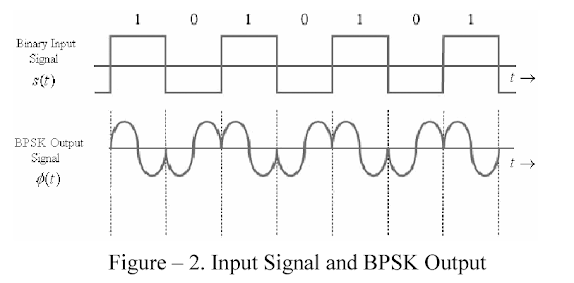
\includegraphics[width=5cm]{./image/BPSK2.png}
% \end{figure}

% Two bits are modulated at ones with the same bandwidth as a 2-PSK so more informations are transmitted at the same time. \cite{Meyer2011}
%TODO: Image Signal Raum 
% Most times there is noise and the points on the constellation diagram become a surface. If the surfaces overlap there will be a problem with decoding. 

\subsection{Quadrature PSK (QPSK)}

\skelpar[2]{QPSK = 4-PSK = 4-QAM}

\section{Multipath fading} \label{sec:multipath-fading}

In the previous section, we discussed how the data is modulated and demodulated at the two ends of the transmission system. This section discusses what happens between the sender and receiver when the modulated passband signal is transmitted wirelessly.

In theory because wireless transmission happens through electromagnetic radiation, to model a wireless channel one would need to solve Maxwell's equations for either the electric or magnetic field, however in practice that is not (analytically) possible. Instead what is typically done, is to model the impulse response of the channel using a geometrical or statistical model, parametrized by a set of coefficients that are either simulated or measured experimentally \cite{Gallager}.

In our relatively simple model we are going to include an additive white Gaussian noise (AWGN) and a Rician (or Rayleighan) fading; both are required to model physical effects of the real world. The former in particular is relevant today, as it mathematically describes dense urban environments.

\subsection{Geometric model}

The simplest way to understand the multipath fading, is to consider it from a geometrical perspective. \figref{fig:multipath-sketch} is a sketch a wireless transmission system affected by multipath fading. The sender's antenna radiates an electromagnetic wave in the direction of the receiver (red line), however even under the best circumstances a part of the signal is dispersed in other directions (blue lines).

\begin{figure}
	\centering
	% vim: set ts=2 sw=2 noet:
\begin{tikzpicture}[
			antenna/.pic = {
				\draw[very thick] (0,0) -- ++(2mm, 3mm) -- ++(-4mm,0) -- cycle;
				\draw[very thick] (0,0) -- ++(0,-5mm) coordinate (-mast) {};
				\draw[thick] (0,0) -- ++(0,3mm);
				\node[inner sep = 0pt, outer sep = 6pt] (-center) at (0,2mm) {};
			},
	]

	% Antennas
	\draw (0,2) pic (T) {antenna} node[above left = 3mm] {\sffamily\bfseries TX};
	\draw (5,0) pic (R) {antenna} node[above right = 3mm] {\sffamily\bfseries RX};

	% wall coefficients
	\draw[thick] (4.75, 2.25) to[out = -20, in = 180] ++(1.2,-.5) node[right] {\(|\Gamma| > 0\)};

	% walls
	\draw[thick, fill = lightgray!20] (3,2) -- ++(2,-.5) -- ++(0,1) -- ++(-2,.5) -- cycle;
	\draw[thick, fill = lightgray!20] (-1,0) -- ++(3,0) -- ++(1,-.5) -- ++(-3,0) -- cycle;


	% reflected signals
	\draw[line width = 2pt, blue!50!white, -latex] (T-center) -- node[above, pos = .5] {\(\tau_2\)} (4,2.25) -- (R-center);
	\draw[line width = 2pt, blue!50!white, -latex] (T-center) -- node[left, pos = .7] {\(\tau_3\)} (1,-.25) -- (R-center);
	\draw[line width = 2pt, blue!50!white, -latex] (T-center) -- node[above, pos = .5] {\(\tau_4\)} (-2.5,1.5) -- (R-center); 

	% another wall
	\draw[thick, fill = lightgray!20] (-2,0) -- ++(-1,.5) -- ++(0,2) --++(1,-.5) -- cycle;

	% LOS path
	\draw[line width = 1mm, red!50!white,
		decorate, decoration = {
			expanding waves, angle = 5, segment length = 2mm
		}
	] (T-center) -- node[above = 2mm, pos = .5] {\(\tau_1\)} (R-center);
\end{tikzpicture}

	\caption{
		Sketch of channel with multipath fading.
		\label{fig:multipath-sketch}
	}
\end{figure}

The problem is that, as is geometrically evident, some paths are longer than others. Because of this fact, the signal is seen by the receiver multiple times with different phase shifts \cite{Gallager,Messier}. To mathematically model this effect, we describe the received signal \(r(t)\) as a linear combination of delayed copies of the sent signal \(s(t)\), each with a different attenuation \(c_k\) and phase shift \(\tau_k\):
\begin{equation} \label{eqn:geom-multipath-rx}
	r(t) = \sum_k c_k s(t - \tau_k).
\end{equation}

The linearity of the model is justified by the assumption that the underlying electromagnetic waves behave linearly (superposition holds) \cite{Gallager}. How many copies of \(s(t)\) (usually referred to as ``taps'' or ``rays'') should be included in \eqref{eqn:geom-multipath-rx}, depends on the precision requirements of the model.

A further complication arises, when one end (or both) is not stationary. In that case the lengths of the paths change over time, and as a result both the delays \(\tau_k\) as well as the attenuations \(c_k\) become functions of time: \(\tau_k(t)\) and \(c_k(t)\) respectively \cite{Gallager,Messier}. Even worse when the velocity at which the device is moving is high, then Doppler shifts of the electromagnetic wave frequency become non negligible \cite{Gallager}.

\begin{figure}
	\centering
	% vim: set ts=2 sw=2 noet:
\tdplotsetmaincoords{70}{40}
\begin{tikzpicture}[tdplot_main_coords, font = \footnotesize\ttfamily]
	\draw[thick, -latex] (0,0,0) -- node[sloped, midway, below, gray] {Effect of the channel} (7,0,0) node[right] {\(\tau\)};
	\draw[thick, -latex] (0,0,0) -- node[sloped, midway, above, gray] {How the channel changes} (0,7,0) node[right] {\(t\)};
	\draw[thick, -latex] (0,0,0) -- (0,0,2) node[above] {\(h(t,\tau)\)};

	\foreach \y in {1,2,...,4}{
		\draw[dashed, gray] (0,1.5*\y,0) -- ++(7,0,0);
	}

	\foreach \x in {1,2,...,6}{
		\draw[dotted, gray] (\x,0,0) -- ++(0,7,0);
	}

	% draw 4 responses
	\begin{scope}[very thick, -{Circle[fill=white]}]
		\foreach \x/\v in {.8/1, 2.2/2, 2.9/1, 4/4, 5.1/7, 5.8/3}{
			\draw[blue!80!red] (\x,1.5*4,0) -- ++(0,0,\v/3);
		}

		\foreach \x/\v in {.9/2, 2.1/2, 3/1, 4/3, 5/6, 6/3}{
			\draw[blue!60!red] (\x,1.5*3,0) -- ++(0,0,\v/3);
		}

		\foreach \x/\v in {.6/1, 2/1, 2.8/3, 4.1/4, 5.5/4, 6.2/1}{
			\draw[blue!40!red] (\x,1.5*2,0) -- ++(0,0,\v/3);
		}

		\foreach \x/\v in {1.1/2, 1.8/1, 3/2, 3.7/1, 4.8/3, 5.8/1}{
			\draw[blue!20!red] (\x,1.5,0) -- ++(0,0,\v/3);
		}
	\end{scope}
\end{tikzpicture}

	\caption{
		LTV impulse response of a multipath fading channel.
		\label{fig:multipath-impulse-response}
	}
\end{figure}

We have thus observed that the arrangement can be modelled as a linear time-\emph{varying} system (LTV), if the sender or the receiver (or anything else in the channel) is moving, and as a linear time \emph{invariant} (LTI) system if the geometry is stationary. Regardless of which of the two cases, linearity alone is sufficient to approximate the channel as finite impulse response (FIR) filter \cite{Messier}. We can rewrite LTV version of equation \eqref{eqn:geom-multipath-rx} using a convolution product as following:
\begin{align*}
	r(t) = \sum_k c_k(t) s(t - \tau_k(t)) &= \sum_k c_k(t) \int_\mathbb{R} s(\tau) \delta(\tau - \tau_k(t)) \,d\tau \\
		&= \int_\mathbb{R} s(\tau) \sum_k c_k(t) \delta(\tau - \tau_k(t)) \,d\tau = s(\tau) * h(\tau, t),
\end{align*}
obtaining a new function
\begin{equation} \label{eqn:multipath-impulse-response}
	h(\tau, t) = \sum_k c_k(t) \delta(\tau - \tau_k(t)),
\end{equation}
that describes the \emph{channel impulse response} (CIR). This function depends on two time parameters: actual time \(t\) and convolution time \(\tau\). To better understand \(h(\tau, t)\), consider an example shown in figure \ref{fig:multipath-impulse-response}. Each stem represents a weighted Dirac delta, so each series of stems of the same color, along the convolution time \(\tau\) axis, is a channel response at some specific time \(t\). Along the other \(t\) axis we see how the entire channel response changes over time\footnote{In the figure only a finite number of stems was drawn, but actually the weights \(c_k(t)\) of the Dirac deltas change continuously.}. Notice that the stems are not quite aligned to the \(\tau\) time raster (dotted lines), that is because in \eqref{eqn:multipath-impulse-response} not only the weights \(c_k\) but also the delays \(\tau_k\) are time dependent.

\subsection{Spectrum of a multipath fading channel}

With a continuous time channel model we can now discuss the spectral properties of a fading channel since the frequency response is the Fourier transform of the impulse response, mathematically \(H(f, t) = \fourier h(\tau, t)\). In this case however \(h(\tau, t)\) depends on two time variables, but that is actually not an issue, it just means that the frequency response is also changing over time. Hence we perform the Fourier transform with respect to the channel (convolution) time variable \(\tau\) to obtain
\begin{equation} \label{eqn:multipath-frequency-response}
	H(f, t) = \int_\mathbb{R} \sum_k c_k(t) \delta(\tau - \tau_k(t)) e^{-2\pi jf\tau} \, d\tau
	= \sum_k c_k(t) e^{-2\pi jf \tau_k(t)}.
\end{equation}

Equation \eqref{eqn:multipath-frequency-response} shows that the frequency response is a periodic complex exponential, which has some important implications. Notice that if there is only one tap (term), the magnitude of \(H(f, t)\) is a constant (with respect to \(f\)) since \(|e^{j\alpha f}| = 1\). This means that the channels attenuates all frequencies by the same amount, therefore it is said to be a \emph{frequency non-selective} or \emph{flat fading} channel. Whereas in the case when there is more than one tap, the taps interfere destructively at certain frequencies and the channel is called \emph{frequency selective}. To illustrate how this happens, plots of the frequency response of a two tap channel model are shown in \figref{fig:multipath-frequency-response-plots}. On the left is the magnitude of \(H(f, t)\), which presents periodic ``dips'', and on the right complex loci for the two taps (red and blue), as well as their sum (magenta), over the frequency range near the first dip (2 to 2.5 MHz) are shown.


\begin{figure}
	\centering
	\resizebox{\linewidth}{!}{
		% vim: set ts=2 sw=2 noet:
\begin{tikzpicture}
	\begin{loglogaxis}[
			width = .6\linewidth, height = 5cm,
			ylabel = {Response \(|H(f, t)|\)},
			xlabel = {Frequency \(f\)/Hz},
			xlabel near ticks,
			ylabel near ticks,
			ytick = \empty,
			smooth,
		]

		\addplot[solid, magenta] table[x index = 0, y index = 2]
			{figures/data/multipath_frequency_response.dat};
		% \addlegendentry{Multipath}

		% \addplot[dashed, thick, black] table[x index = 0, y index = 1]
		% 	{figures/data/multipath_frequency_response.dat};
		% \addlegendentry{Linear}

	\end{loglogaxis}
\end{tikzpicture}
\hskip 5mm
\begin{tikzpicture}[
		decorated/.style = {
			solid, thick,
			postaction={decorate},
			decoration={markings,
				mark=at position 0.35 with {\arrow{stealth}},
				mark=at position 0.65 with {\arrow{stealth}}},
		},
	]
	\begin{axis}[
			width = 5cm, height = 5cm,
			ylabel = {\(\Im{H(f,t)}\)},
			xlabel = {\(\Re{H(f,t)}\)},
			xlabel near ticks,
			ylabel near ticks,
			grid = major,
			xmin = -1.2, xmax = 1.2,
			ymin = -1.2, ymax = 1.2,
		]

		\addplot[decorated, red] table[x index = 3, y index = 4]
			{figures/data/multipath_frequency_response.dat}
			node[pos = 0, circle, fill = white, draw, inner sep = 1pt] {}
			node[pos = .2, outer sep = 1pt, inner sep = 0pt] (A) {}
			node[pos = 1, circle, fill = white, draw, inner sep = 1pt] {};

		\addplot[decorated, blue] table[x index = 5, y index = 6]
			{figures/data/multipath_frequency_response.dat}
			node[pos = 0, circle, fill = white, draw, inner sep = 1pt] {}
			node[pos = .2, outer sep = 1pt, inner sep = 0pt] (B) {}
			node[pos = 1, circle, fill = white, draw, inner sep = 1pt] {};

		\addplot[decorated, magenta] table[x index = 7, y index = 8]
			{figures/data/multipath_frequency_response.dat}
			node[pos = 0, circle, fill = white, draw, inner sep = 1pt] {}
			node[pos = 0, below right, font = \tiny] {2 MHz}
			node[pos = .2, outer sep = 1pt, inner sep = 0pt] (C) {}
			node[pos = 1, circle, fill = white, draw, inner sep = 1pt] {}
			node[pos = 1, above left, font = \tiny] {2.5 MHz};

		\node[outer sep = 2pt, inner sep = 0pt] (O) at (0,0) {};
		\draw[-latex, red!50!white] (O) -- (A);
		\draw[-latex, blue!50!white] (O) -- (B);
		\draw[-latex, magenta!50!white] (O) -- (C);

	\end{axis}
\end{tikzpicture}

		% \skelfig[width = .8 \linewidth, height = 3cm]{}
	}
	\caption{
		Frequency response of a multipath fading channel.
		\label{fig:multipath-frequency-response-plots}
	}
\end{figure}

\subsection{Quantifying dispersion}

Having discussed how multipath fading affects communication systems, the next important step is to be able quantify its effects to be able to compare different multipath channels to each other.

An intuitive parameter to quantify how dispersive channel is, is to take the time difference between the fastest and slowest paths with significant energy. What in the literature is called \emph{delay spread}, and is denoted here by \(T_d\). Consequently, a low delay spread means that all paths have more or less the same length, while a high delay spread implies that there is a large difference in length among the paths. Thus \(T_d\) could be be defined as
\begin{equation}
	T_d = \max_{k} (\tau_k(t)) -  \min_{k} (\tau_k(t)),
\end{equation}
as is done in \cite{Gallager}. However since in reality some paths get more attenuated than others (\(c_k(t)\) parameters) it also not uncommon to define the delay spread as a weighted mean or even as a statistical second moment (RMS value), where mean tap power \(\expectation\{|c_k(t)|^2\}\) is taken into account \cite{Mathis,Messier}. More sophisticated definitions of delay spread will be briefly mentioned later in section \ref{sec:statistical-model}.

Another important parameter for quantifying dispersion is \emph{coherence bandwidth}, a measure how 
\skelpar{sentence}

% TODO: End the sentence

\subsection{Effects of multipath fading on modulation constellations}

% TODO : Can we sai it that way /dose it need to be in the implementation Part?

It is to mention that not every constellation of parameter for a fading illustration leads to a satisfying  plot constellation.
For example in a Discrete-time Model: the same delay as the samples per Symbol or a multiple of it leads to a special case, where we see the constellation are around the modulate signal points, when there is no line of side path. This is because of \skelpar{Beschreiben warnn die Werte hübsch sind}

\subsection{Discrete-time model} \label{sec:discrete-time-model}

% TODO: discuss the "bins" of discrete time

Since in practice signal processing is done digitally, it is meaningful to discuss the properties of a discrete-time model. To keep the complexity of the model manageable some assumptions are necessary, thus the sent discrete signal\footnote{This is an abuse of notation. The argument \(n\) is used to mean the \(n\)-th digital sample of \(s\), whereas \(s(t)\) is used for the analog waveform. A more correct but longer notation is \(s(nT)\), where \(T\) is the sample time.} \(s(n)\) is assumed to have a finite single sided bandwidth \(W\). This implies that in the time-domain signal is a series of sinc-shaped pulses each shifted from the previous by a time interval \(T = 1 / (2W)\) (Nyquist rate):
\begin{equation}
	s(t) = \sum_n s(n) \sinc(t/T - n)
\end{equation}
The waveform \(s(t)\) is then convolved with the CIR function \(h(\tau, t)\) (with respect to \(\tau\)) from the continuous time model resulting in the waveform at the receiver
\begin{align*}
	r(t) &= \int_ \mathbb{R} \sum_n s(n) \sinc(\tau / T - n) \sum_k c_k(t) \delta(\tau - \tau_k(t)) \,d\tau \\
	&= \sum_n s(n) \sum_k c_k(t) \sinc(t/T - \tau_k(t)/T - n),
\end{align*}
which is then sampled at the Nyquist rate of \(2W = 1/T\), resulting in a set of samples\footnote{Again, the abusing notation \(r(m)\) means the \(m\)-th digital sample of \(r(t)\), i.e. \(r(mT)\).}:
\[
	r(m) = \sum_n s(n) \sum_k c_k(mT) \sinc(m - \tau_k(mT)/T - n).
\]
Finally the substitution \(l = m - n\) eliminates the sender's sample counter \(n\) (unknown to the receiver) and reformulates \(r(m)\) as a discrete convolution product of with a discrete CIR function \(h_l(m)\):
\begin{equation}
	r(m) = \sum_l s(m - l) \sum_k c_k(mT) \sinc(l - \tau_k(mT)/T) 
	= \sum_l s(m - l) h_l (m).
\end{equation}
This result is very similar to the continuous time model described by \eqref{eqn:multipath-impulse-response} in the sense that each received digital sample is a sent sample convolved with a different discrete channel response (because of time variance). To see how the discrete CIR
\begin{equation} \label{eqn:discrete-multipath-impulse-response}
	h_l(m) = \sum_k c_k(mT) \sinc(l - \tau(mT)/T)
\end{equation}
is different from \eqref{eqn:multipath-impulse-response} consider again the plot of \(h(\tau,t)\) in \figref{fig:multipath-impulse-response}. The plot of \(h_l(m)\) would have discrete axes with \(m\) replacing \(t\) and \(l\) instead of \(\tau\), and because of the finite bandwidth in the \(l\) axis instead of Dirac deltas there would be superposed sinc functions.

\begin{figure}
	\centering
	% vim: set ts=2 sw=2 noet:
\begin{tikzpicture}[
		dot/.style = {
			circle,
			fill = black, draw = black,
			minimum size = 1.5mm,
			outer sep = 0, inner sep = 0,
		},
		block/.style = {
			rectangle, draw, thick,
			black, fill = white,
			minimum height = 8mm, minimum width = 8mm,
		},
		prod/.style = {
			circle, draw, thick,
			black, fill = white,
			minimum size = 6mm,
			inner sep = 0, outer sep = 0,
		},
		sum/.style = {
			circle, draw, thick,
			black, fill = white,
			minimum size = 6mm,
			inner sep = 0, outer sep = 0,
		},
	]

	\matrix[column sep = 5mm, row sep = 3mm] {
		\node[block] (B0) {\(z^{-1}\)}; & \node[dot] (D0) {}; &
		\node[block] (B1) {\(z^{-1}\)}; & \node[dot] (D1) {}; &
		\node[block] (B2) {\(z^{-1}\)}; & \node[dot] (D2) {}; & \node (dots) {\ldots}; & 
		\node[block] (Bk) {\(z^{-1}\)}; &
		\\
		& \node[prod] (P0) {\(\times\)}; &
		& \node[prod] (P1) {\(\times\)}; &
		& \node[prod] (P2) {\(\times\)}; & &
		& \node[prod] (Pk) {\(\times\)}; &
		\\[6mm]
		& & & & & & & & \node[sum] (S) {\(+\)}; \\
	};

	\begin{scope}[thick, -latex]
		% delayed line
		\draw[latex-] (B0.west) -- ++(-5mm,0) node[left] {\(s(n)\)};
		\draw (B0.east) -- (D0) -- (B1.west);
		\draw (B1.east) -- (D1) -- (B2.west);
		\draw (B2.east) -- (D2) -- (dots) -- (Bk.west);

		% taps
		\draw (D0) -- (P0);
		\draw (P0) |- (S);

		\draw (D1) -- (P1);
		\draw (P1.south) |- ($(S) + (150:10mm)$) -- (S);

		\draw (D2) -- (P2);
		\draw (P2.south) |- ($(S) + (120:10mm)$) -- (S);

		\draw (Bk) -| (Pk);
		\draw (Pk) -- (S);

		% product weights
		\draw[latex-] (P0.west) -- ++(-4mm,0) node[left] {\(h_1(m)\)};
		\draw[latex-] (P1.west) -- ++(-4mm,0) node[left] {\(h_2(m)\)};
		\draw[latex-] (P2.west) -- ++(-4mm,0) node[left] {\(h_3(m)\)};
		\draw[latex-] (Pk.west) -- ++(-4mm,0) node[left] {\(h_l(m)\)};

		% result
		\draw (S.south) |- ++(1cm,-3mm) node[right] {\(r(m)\)};
	\end{scope}

\end{tikzpicture}

	\caption{
		Fading channel as a tapped delay line.
		\label{fig:tapped-delay-line}
	}
\end{figure}

From a signal processing perspective \eqref{eqn:discrete-multipath-impulse-response} can be interpreted as a simple tapped delay line, schematically drawn in \figref{fig:tapped-delay-line}, which confirms that the presented mathematical model is indeed a FIR filter. Simple multipath channels can be simulated with just a few lines of code, for example the data for the static fading channel in \figref{fig:multipath-frequency-response-plots} is generated in just four lines of Python. The difficulty of fading channels in practice lies in the estimation of the constantly changing parameters \(c_k(t)\) and \(\tau_k(t)\).


\subsection{Simulating multipath CIR with FIR filters} \label{sec:fractional-delay}
% TODO quelle: http://users.spa.aalto.fi/vpv/publications/vesan_vaitos/ch3_pt1_fir.pdf

\begin{figure}
	\centering
	\begin{subfigure}{.45\linewidth}
		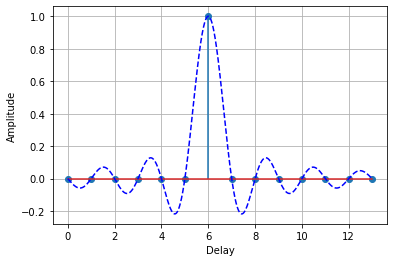
\includegraphics[width=\linewidth]{./figures/screenshots/Fractional_delay_6}
		\caption{Pulse with an integer delay of 6 samples.}
	\end{subfigure}
	\hskip 5mm
	\begin{subfigure}{.45\linewidth}
		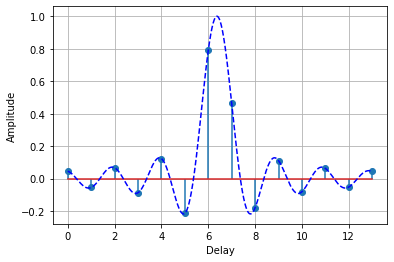
\includegraphics[width=\linewidth]{./figures/screenshots/Fractional_delay_637}
		\caption{Pulse with a fractional delay of 6.37 samples.}
	\end{subfigure}
	\caption{\label{fig:fractional-delay-sinc-plot}}
\end{figure}

As mentioned in \ref{sec:discrete-time-model} a FIR filter can be used to simulate discrete-time models of multipath fading. But with FIR filters the delays can only be integer multiples of the sample rate. When the delays are non integer an approximation needs to be done, that is because FIR filters have a transfer function of the form
\begin{equation} \label{eqn:transfer-function-fir}
	H(j\omega) = \sum_{n = 0}^{N} h(n) e^{-j\omega nT}
	\quad \text{commonly written as} \quad
	H(z) = \sum_{n = 0}^{N} h(n) z^{-n},
\end{equation}
but a non integer delay of \(\tau\) in the frequency domain is \(H_\tau(j\omega) = e^{-j\omega \tau}\). There are multiple ways to find coefficients \(h(n)\) that approximate \(H_\tau\), in this case the least squares method was used by minimizing the error function
\begin{equation}
	E(j\omega) = H(j\omega) - H_\tau(j\omega).
\end{equation}
The least square method plus the assumption of finite bandwidth and the requirement of causality gives the following rule for computing the FIR filter coefficients:
\begin{equation}
	h(n)= \begin{cases}
		\sinc (n - \tau) & 0 \leq n \leq N \\ 
		0 & \text { otherwise }
	\end{cases},
\end{equation}
where the odd order of the filter \(N\) should satisfy the condition
\begin{equation} \label{eqn:fractional-fir-length}
	N = 2 \lfloor \tau \rfloor + 1
\end{equation}
for a minimal error in the approximation. It is worth mentioning that it is also possible to build FIR filters of even length with a different condition, or that do not satisfy \eqref{eqn:fractional-fir-length}, in which cases more consideration is required. An example of a fractional delay FIR filter is shown in \figref{fig:fractional-delay-sinc-plot}.

\subsection{Statistical model} \label{sec:statistical-model}
%TODO: Quelle?
Because as mentioned earlier it is difficult to estimate the time-dependent parameters of \(h_l(m)\) in many cases it is easier to model the components of the CIR as stochastic processes, thus greatly reducing the number of parameters. This is especially effective for channels that are constantly changing, because by the central limit theorem the cumulative effect of many small changes tends to a normal distribution.

Recall that \(h_l(m)\) is a function of time because \(c_k\) and \(\tau_k\) change over time. The idea of the statistical model is to replace the cumulative change caused by \(c_k\) and \(\tau_k\) (which are difficult to estimate) by picking the next CIR sample \(h_l(m +1)\) from a \emph{circularly symmetric complex Gaussian distribution}, or concisely written as
\begin{equation}
	h_l \sim \mathcal{CN}(0, \sigma^2)
\end{equation} 
for some parameter \(\sigma\). Loosely speaking, the distribution needs to be ``circular'' because \(h_l\) is a complex number, which is a ``two dimensional number'', it can however be understood as \(\Re{h_l} \sim \mathcal{N}(0, \sigma^2)\) and \(\Im{h_l} \sim \mathcal{N}(\mu, \sigma^2)\), i.e. having each component being normally distributed.


%TODO : Picture of gaussian distribution
\begin{subequations}
	\begin{align}
		R_{l} (k) &= \E{h_l(m) h_l^*(m+k)}, \\
		0 &= \E{h_l(m) h_k^*(m)} \text { for } l \neq k
	\end{align}
\end{subequations}

\begin{figure}
	\centering
	\begin{subfigure}{.45\linewidth}
		\skelfig
		\caption{NLOS, Rayleigh}
	\end{subfigure}
	\hskip 5mm
	\begin{subfigure}{.45\linewidth}
		\skelfig 
		\caption{LOS, Rice}
	\end{subfigure}
	\caption{
		Ring of scattering objects.
		\label{fig:multipath-statistical-models}
	}
\end{figure}

%TODO :Maby some correction on the descreption, because mentionet earlyer Is f(t) =(c k (t) parameters)?
\paragraph{NLOS case}

 In the case of the Rayleight distribution the signal has no line of sight. It can be looked at the Fading process \cite{Hoher2013} with the help of the amplitude \(a(t)\) in time and the associated phase \(\Theta(t) \in[\,0,2\pi)\,\). To find the probability function of the amplitutes it can be looked at the fading possess as a superimposition of those infinity distribute signals:
\begin{equation} \label{eqn:rayleight fading}
 	f(t) = \lim_{N\rightarrow\infty} \frac{1}{\sqrt{N}}\sum_{n=1}^{N} e^{j(\Theta +2\pi jf t)}.
 \end{equation}  
whish are nominate with the factor \(\frac{1}{\sqrt{N}}\) so that the power probability is \(\E{|f(t)|²}=1\) as mentioned earlier. From the fact that we are looking at the complex basiband and this processes is an independent one with a gaussian distributions it can be said that \(\E{f(t)}=0\) and so the propabiliti of the amplitude is:
 
\begin{equation} \label{eqn:rayleight_fading_probabilety_dencety}
	p(a)= 2a\exp{{-a}^2}
\end{equation}

It can also explaint with I- and Q-contribution :
\begin{equation}
	\Re{h_l(n)}, \Im{h_l(n)}
	\sim \mathcal{N} \left(0, \frac{1}{2} \E{|h_l(n)|^2} \right)
\end{equation}
\skelpar[4]

\paragraph{LOS case}
In the case of the Rician distribution model. The line of side exist, which means that one of the paths have a straight communication line from the transmitter to the reviser.

It can be said that a Rayleight distribution is the same as a Rician distribution with a factor K =0.

For a faktor K= 5.1 the probability function is gaussien distributed.

\skelpar[4]{Explain statistical model with Rician distribution.}
\begin{equation}
	\Re{h_l(n)}, \Im{h_l(n)}
	\sim \mathcal{N} \left( \frac{A_l}{\sqrt{2}}, \frac{1}{2} \sigma_l^2 \right)
\end{equation}
\skelpar[4]

	% vim: set ts=2 sw=2 noet spell:

\chapter{Implementation}

\section{Overview}

% TODO: quelle https://wiki.gnuradio.org/
For the simulation task and after for the Hardware part, the open-source Software GNU Radio has been chosen. This software uses toolboxes for signal processing systems too simulate or/and implement a software-defined radio, based on Python and some C++ implementations for some rapid-application-development environments. The toolboxes can simply, with the help of the graphical user interface, used by drag-and-drop. The Boxes are used to write applications, to receive or to transmit date for a digital system. Some blocks like different filters, channel codes or demodulator elements and a lot more are already implemented. For missing application new elements can be added by coding own blocks. With the help of the GNU Radio software those toolboxes can easily get connected to each other, creating data streams. 

\section{Sender chain}
\subsection{Data source}

%% TODO: replace with file file
In this simulation a random source has been chosen.

\subsection{Modulation}

The constellation modulator block is used for a root-raised-cosine-filtered basis modulation. The block gives an input of a byte stream as complex modulated signal in the baseband back. 
Further more it's possible to chose the modulation type here, in this example it is 16QAM, but QPSK, 8PSK and BPSK would also be possible.

\section{Receiver chain}

\subsection{Envelope detector}

\paragraph{Polyphase Clock Sync}
%% To Do : nochmals anschauen ob dieese erklärung verständlich ist und richtig interpretiert wurde.
With the the polyphase clock sync the symbols can be synchronized by preforming a time synchronization with the help of multiple filterbanks. For that the derivation of the filtered signal should be minimized whish turns to a better SNR. This works with the help of two filterbanks, one of them contains the filters of the signal adapted to the pulse shaping with several phases. The other contains its derivative. So in the time domain it has a sinc shape, for the output Signal the sinc peak should be on a sample, with the fact that sinc(0) = 1 and sinc(0)' = 0 an error signal can be generated which tells how far away from the peak it is. This error Signal should be zero this is possible with the help of a loop second order whish constants the number of the filterbank and the rate. This rate is generated because of the clock difference between the transmitter and reviver to synchronies the receiver the filter goes through the phases. For the output one sample per symbol is enough.

\paragraph{Equalizer}

\paragraph{Costas Loop}

The Costas Loop is used for frequency and phase adjustment it locks the center frequency of the signal additional it converts it back to de baseband.  For different modulation types different orders of the loop had to be chosen 

\paragraph{Constellation decoder}

From the complex space the constellation points are decode to bits.

\subsection{Frame synchronization}

\begin{figure}
	\centering
	% vim:ts=2 sw=2:
\begin{tikzpicture}[
		brace/.style = {
			decorate,
			decoration = {
				calligraphic brace,
				amplitude = 3mm,
				raise = 1mm,
				mirror,
			},
			very thick,
			pen colour = {black} 
		},
	]
	\matrix[
		column sep = -1pt,
		nodes = {
			draw, rectangle, very thick,
			minimum height = 12mm,
			text width = 20mm,
			align = center,
		},
	]{
		\node[] {Preamble \\ \(k\) Bytes}; &
		\node[fill=lightgray!20] (pad) {Padding \\ 1 Bit}; &
		\node[fill=red!10] (id) {ID \\ 5 Bits}; &
		\node[fill=red!10] {Length \\ 21 Bits}; &
		\node[fill=red!10] (par) {Parity \\ 5 Bits}; &
		\node[] {Payload \\ \(\ell\) Bytes}; \\
		% \node{Padding }; \\
	};

	\draw[brace] (id.south west) --
		node[midway, below = 5mm] {(31, 26) Hamming ECC}
		(par.south east);

	% \draw[brace] (par.north east) --
	% 	node[midway, above = 5mm] {4 Bytes}
	% 	(pad.north west);

\end{tikzpicture}

	\caption{
		Structure of framed data packets used in the implementation.
		\label{fig:dataframe}
	}
\end{figure}

To compute the empirical \emph{bit error rate} (BER) of the setup, the data has to be framed on by the sender and the bitstream synchronized on the receiver side. The structure of a data packed used in the implementation is shown in \figref{fig:dataframe}. A frame begins with an user specified \(k\)-byte preamble, that in the current implementation serves as synchronization pattern. Another use case for the preamble sequence could be to introduce channel estimation pilot symbols. Following the preamble are 4 bytes encoded using a (31, 26) Hamming code (plus 1 padding bit), that contain metadata about the packet, namely payload ID and payload length. Because the payload length in bytes is encoded in 21 bits, the maximum payload size is 2 MiB, which together with 32 possible unique IDs gives a maximum data transfer with unique frame headers of 64 MiB. These constraints are a result of decisions made to keep the implementation simple.

On the receiver side the bitstream is synchronized using a XOR correlator. To find the synchronization delay \(d\) (in samples) the XOR correlator computes the binary cross correlation
\begin{equation} \label{eqn:binary-xcorr}
	R_{\vec{m}\vec{p}} = N - \sum_i (\vec{m} \oplus \vec{p})_i
\end{equation}
between the synchronization bit pattern \(\vec{p}\) and a shift register \(\vec{m}(n)\) of the same length \(N\). Put into words \eqref{eqn:binary-xcorr} subtracts the number bits that differ between \(\vec{m}\) and \(\vec{p}\) from the length of the registers. Thus if all bits are equal, the difference is zero and the correlations has a maximum value of \(N\). The task of the correlator is then to find the delay / skip such that the pattern maches, i.e.
\begin{equation}
	d = \argmax_n \big( R_{\vec{m}\vec{p}}(n) \big)
		= \argmax_n \left( N - \sum_i (\vec{m}(n) \oplus \vec{p})_i \right)
	.
\end{equation}

Once the bit stream is synchronized, the packets are deframed and the payloads compared to a local copy of the sent data to compute the BER, again by XOR'ing the data blocks and counting the bit that are set. Further details are discussed in \S\ref{sec:ber}.

\section{Channel simulations}

Here its possible to add some AWGN noise in the channel line. Different parameters can be changed like the noise voltage, time or the frequency offset.

\skelpar[5]{
	Discuss the multitap FIR model we used. How it is possible to set the delay etc. Also mathematics for the interpolation.
}

%To get a basic line for further simulations a 16QAM has been made. The results of this simulation are shown in \figref{fig:simul16QAM} and \figref{fig:simul16QAM_1} as the red Signal. In \tabref{tab:modulation_settings} some importer Parameter settings for a different modulation scheme are mentioned.
%
%A FIR-Filter was added in the Channel to create a time delay between tow paths. In \figref{fig:simul16QAM} the result includes a direct path and a delayed one. In the plot of \figref{fig:simul16QAM_1} the transmission line dosn't include a direct path. %It's impotent to mention that the delay should be smaller than the symbol rate or a multiple of it. (Stimmt dies , not sure any more)
%
%For the a first simulation with some fading the 16QAM simulation model has been extended with a FIR-Filter in the Chanel. The results of this simulation are shown in \figref{fig:simul16QAM} and \figref{fig:simul16QAM_1} as the blue Signal.

\subsection{Fading}
%TO DO: übersetzen 
Für die statische implementation und veranschaulichen des Fading effekts wurde ein eigener Block kreaiert und in den Channel implementiert. Dieser Block basiert auf einem FIR Filter. Es kann mit direcktem Pfad oder ohne dargestellt werden (Line of Side). Mit Hilfe dieses Filters wird die Verspätung der nebenpfaden dargestellt. Es ist möglich beliebig viele dieser Pfade mit unterschiedlicher stärke zu simulieren. Dieser Block wurde zusätzlich mit der methode in \ref{sec:fractional-delay} beschriben implementiert um nichtganzahlige delay werte zu erlauben.

% Bild einfügen 





\section{Hardware}

As Hardware we chosen the USRP B210 from Ettus Research, with the following specifications shown in \tabref{tab:USRP B210 specifications}. Because this SDR is more than enough for our requires.

For the Hardware setup up some changes are made in the file from the 16QAM simulation to fit with the SDRs. For the first test a coaxial cable was used as transmission line, after the cabel were been replaced with two antennas. The gnu radio block scheme is shown in \figref{fig:simul16QAM_Hardware_Aufbau}. The results for s anntena set uo with a transmission line of 20cm  are plotted in \figref{fig:simul16QAM__Hardware}.

Instead of the channel modeling block the USRP blocks are used. The sink as transmitter and the source as resiver.  The Signal is sended on a center frequency of 2.4GHz.

\subsection{Empirical BER} \label{sec:ber}

\subsection{Measurements}

%
%
%

\begin{figure}
	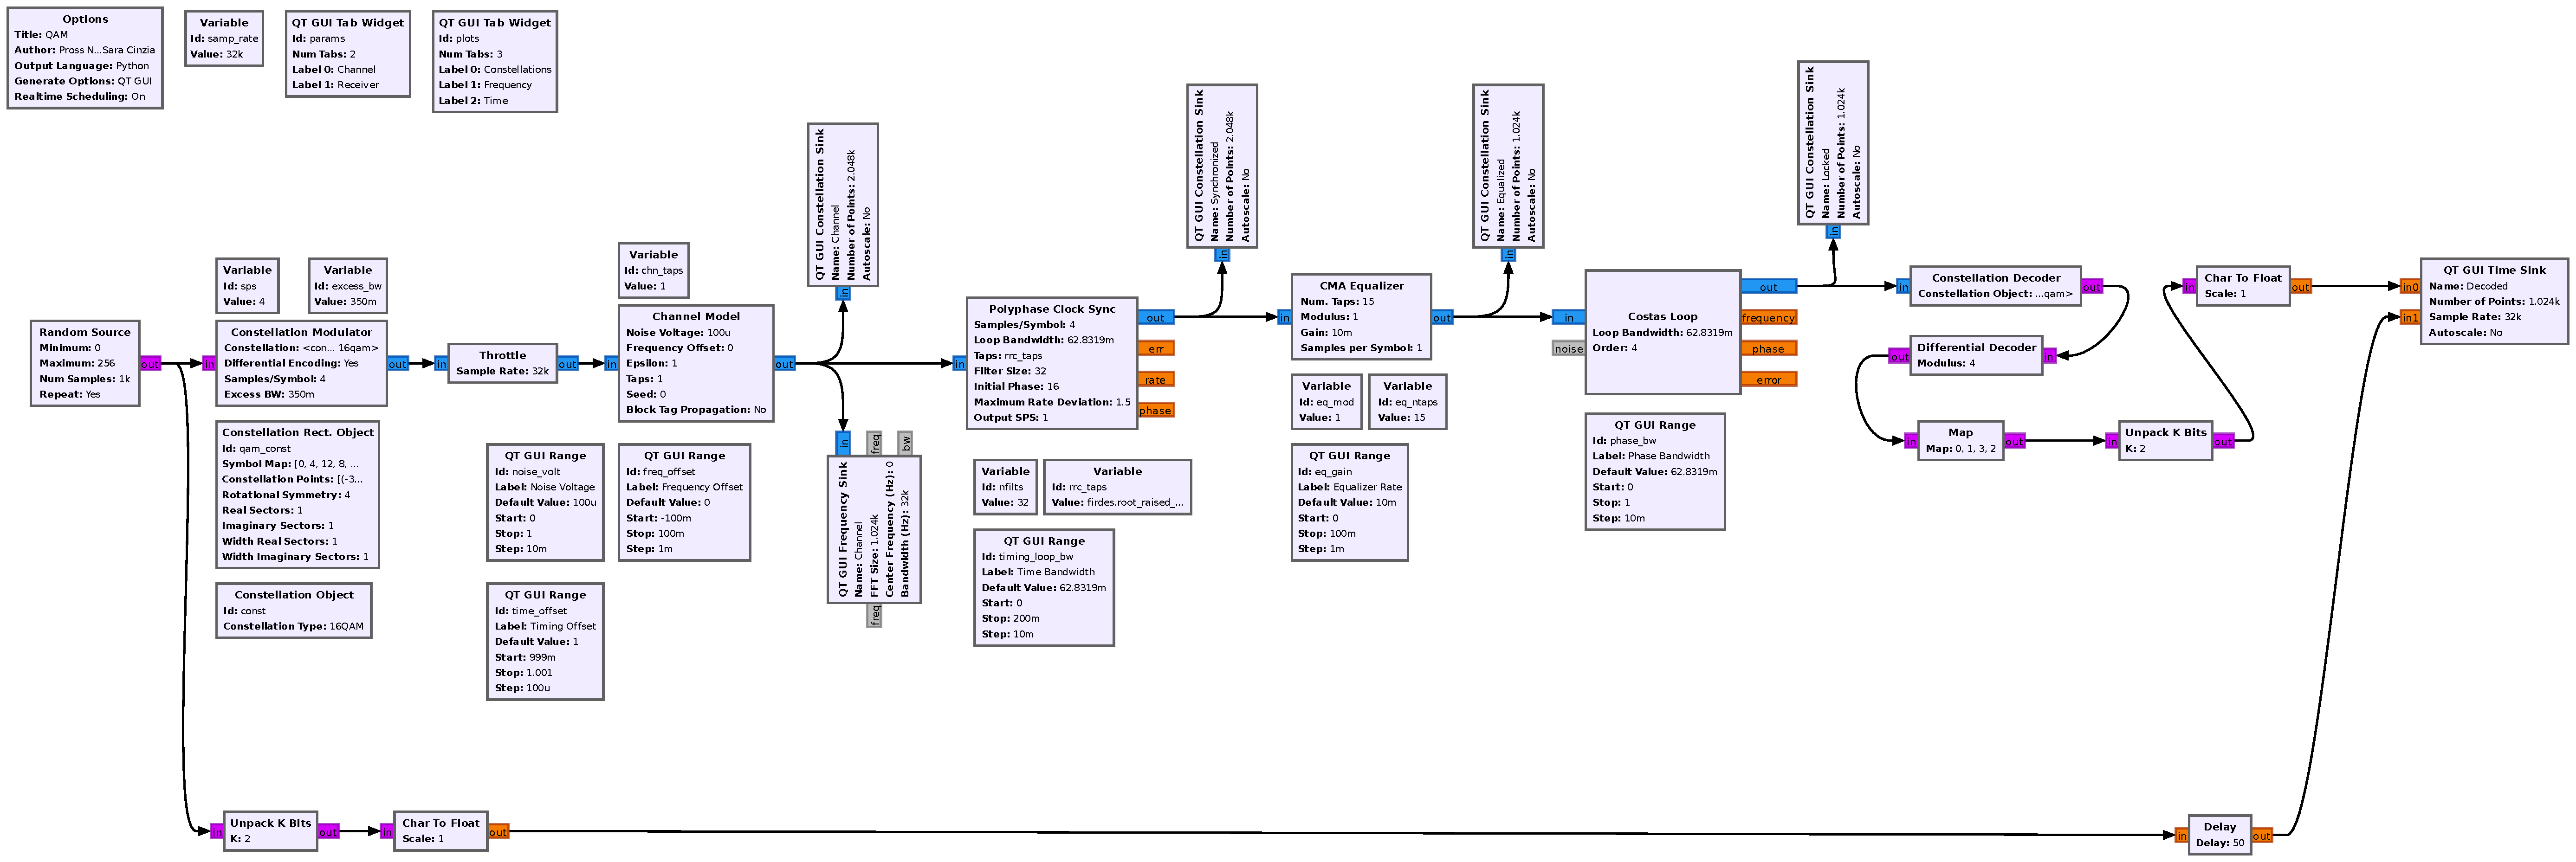
\includegraphics[width=\linewidth]{./figures/pdfs/qam_nogui.pdf}
	\caption{GNU Radio Blocks}
	\label{fig:simul16QAM_block}	
\end{figure}

\begin{figure}
	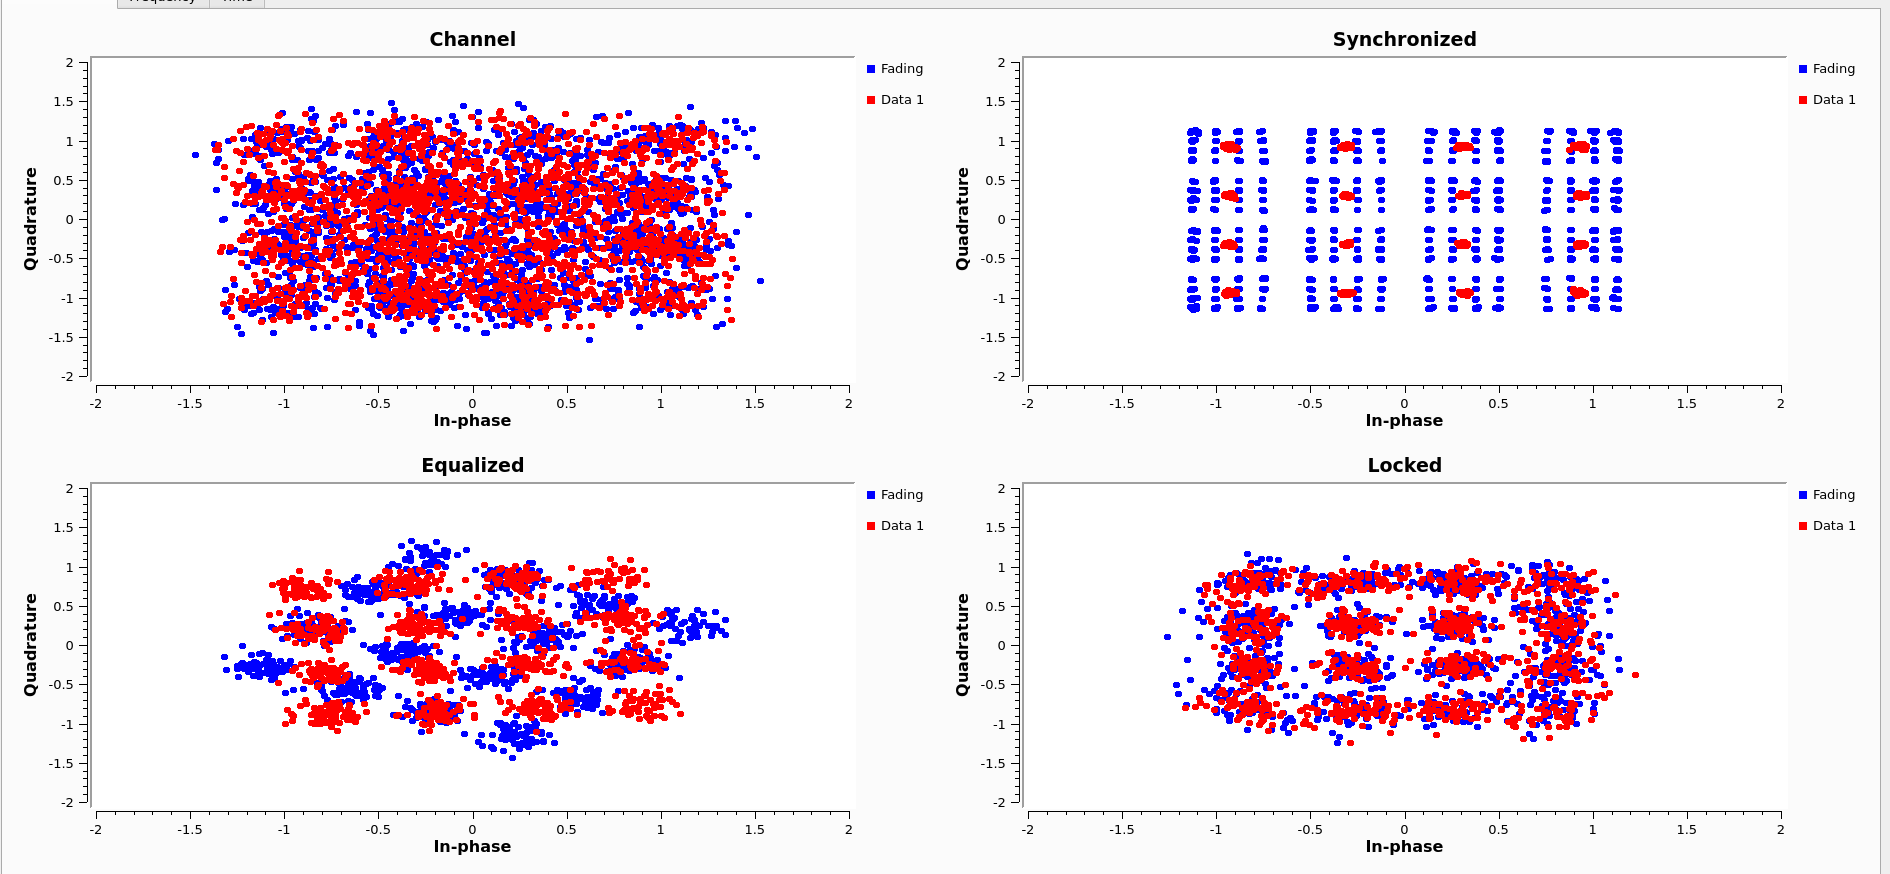
\includegraphics[width=\linewidth]{./figures/screenshots/QAM16_Fading_2.png}
	\caption{Simulation results}
	\label{fig:simul16QAM}	
\end{figure}

\begin{figure}
	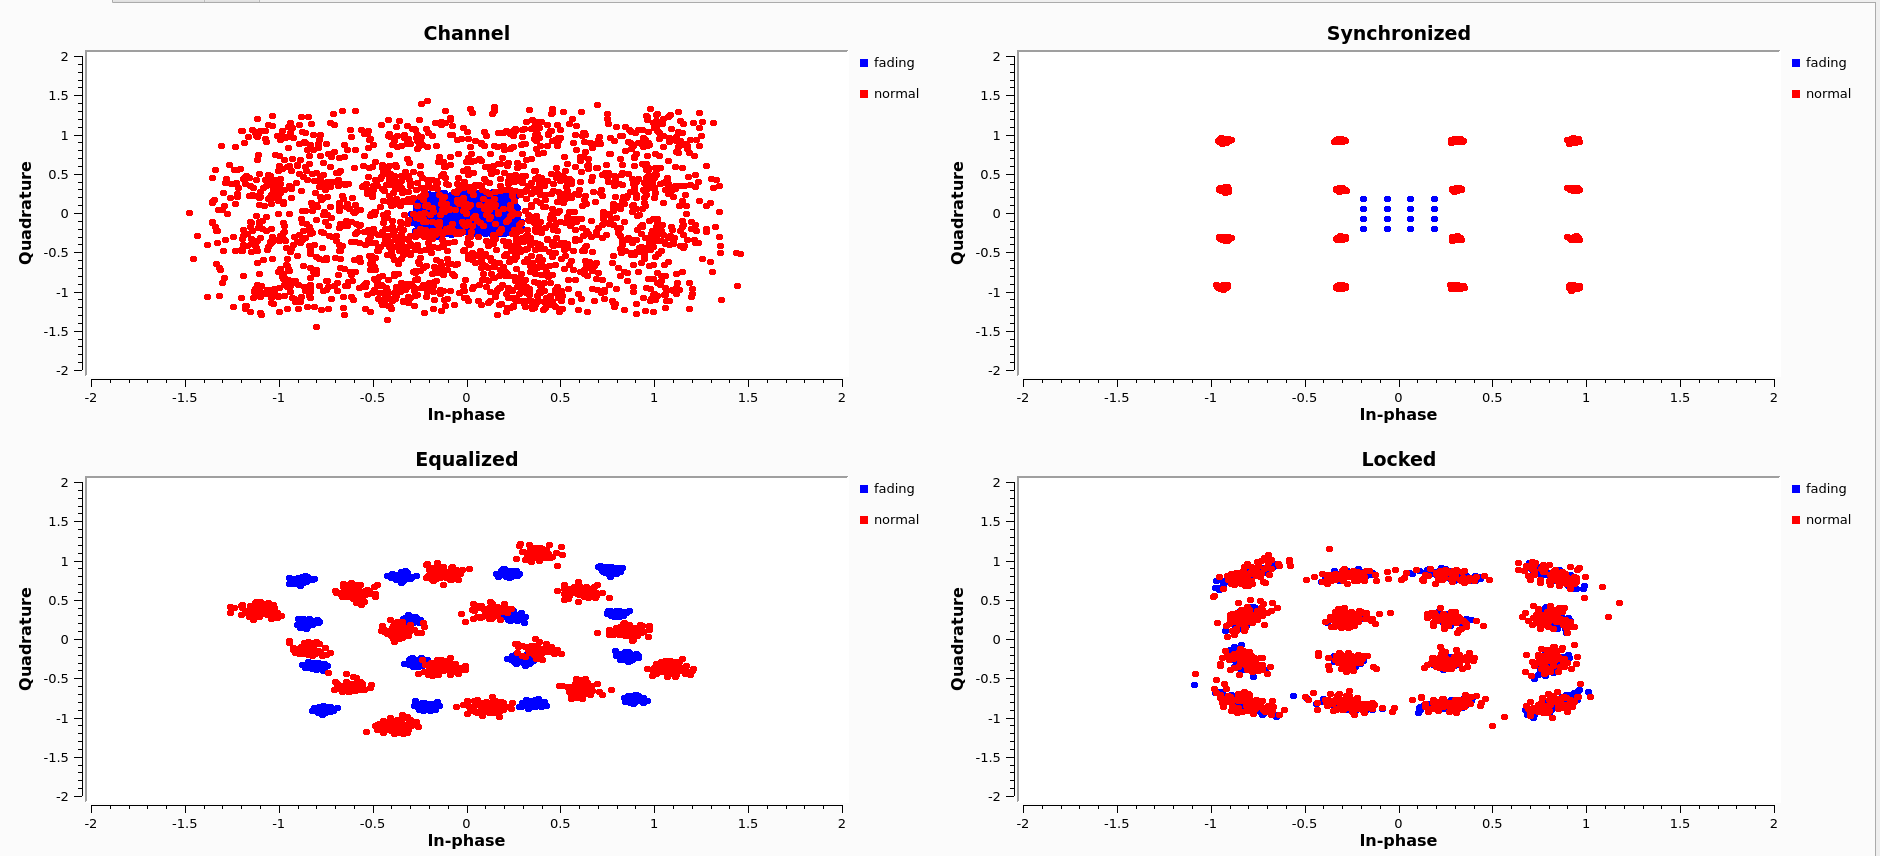
\includegraphics[width=\linewidth]{./figures/screenshots/QAM16_Fading_2_.png}
	\caption{Simulation results}
	\label{fig:simul16QAM_1}	
\end{figure}

\begin{table}[]
	\centering
	\caption{Modulation settings for different scheme}
	\begin{tabular}{ccc}
		\toprule
		Modulation Scheme & Samples per Symbol & Costas Loop Order\\
		\midrule
		BPSK  & 1 & 2 \\
		QPSK  & 2 & 4 \\
		8PSK  & 3 & 8 \\
		16QAM & 4 & 4 \\
		\bottomrule
	\end{tabular}
	\label{tab:modulation_settings}
\end{table}

\begin{figure}
	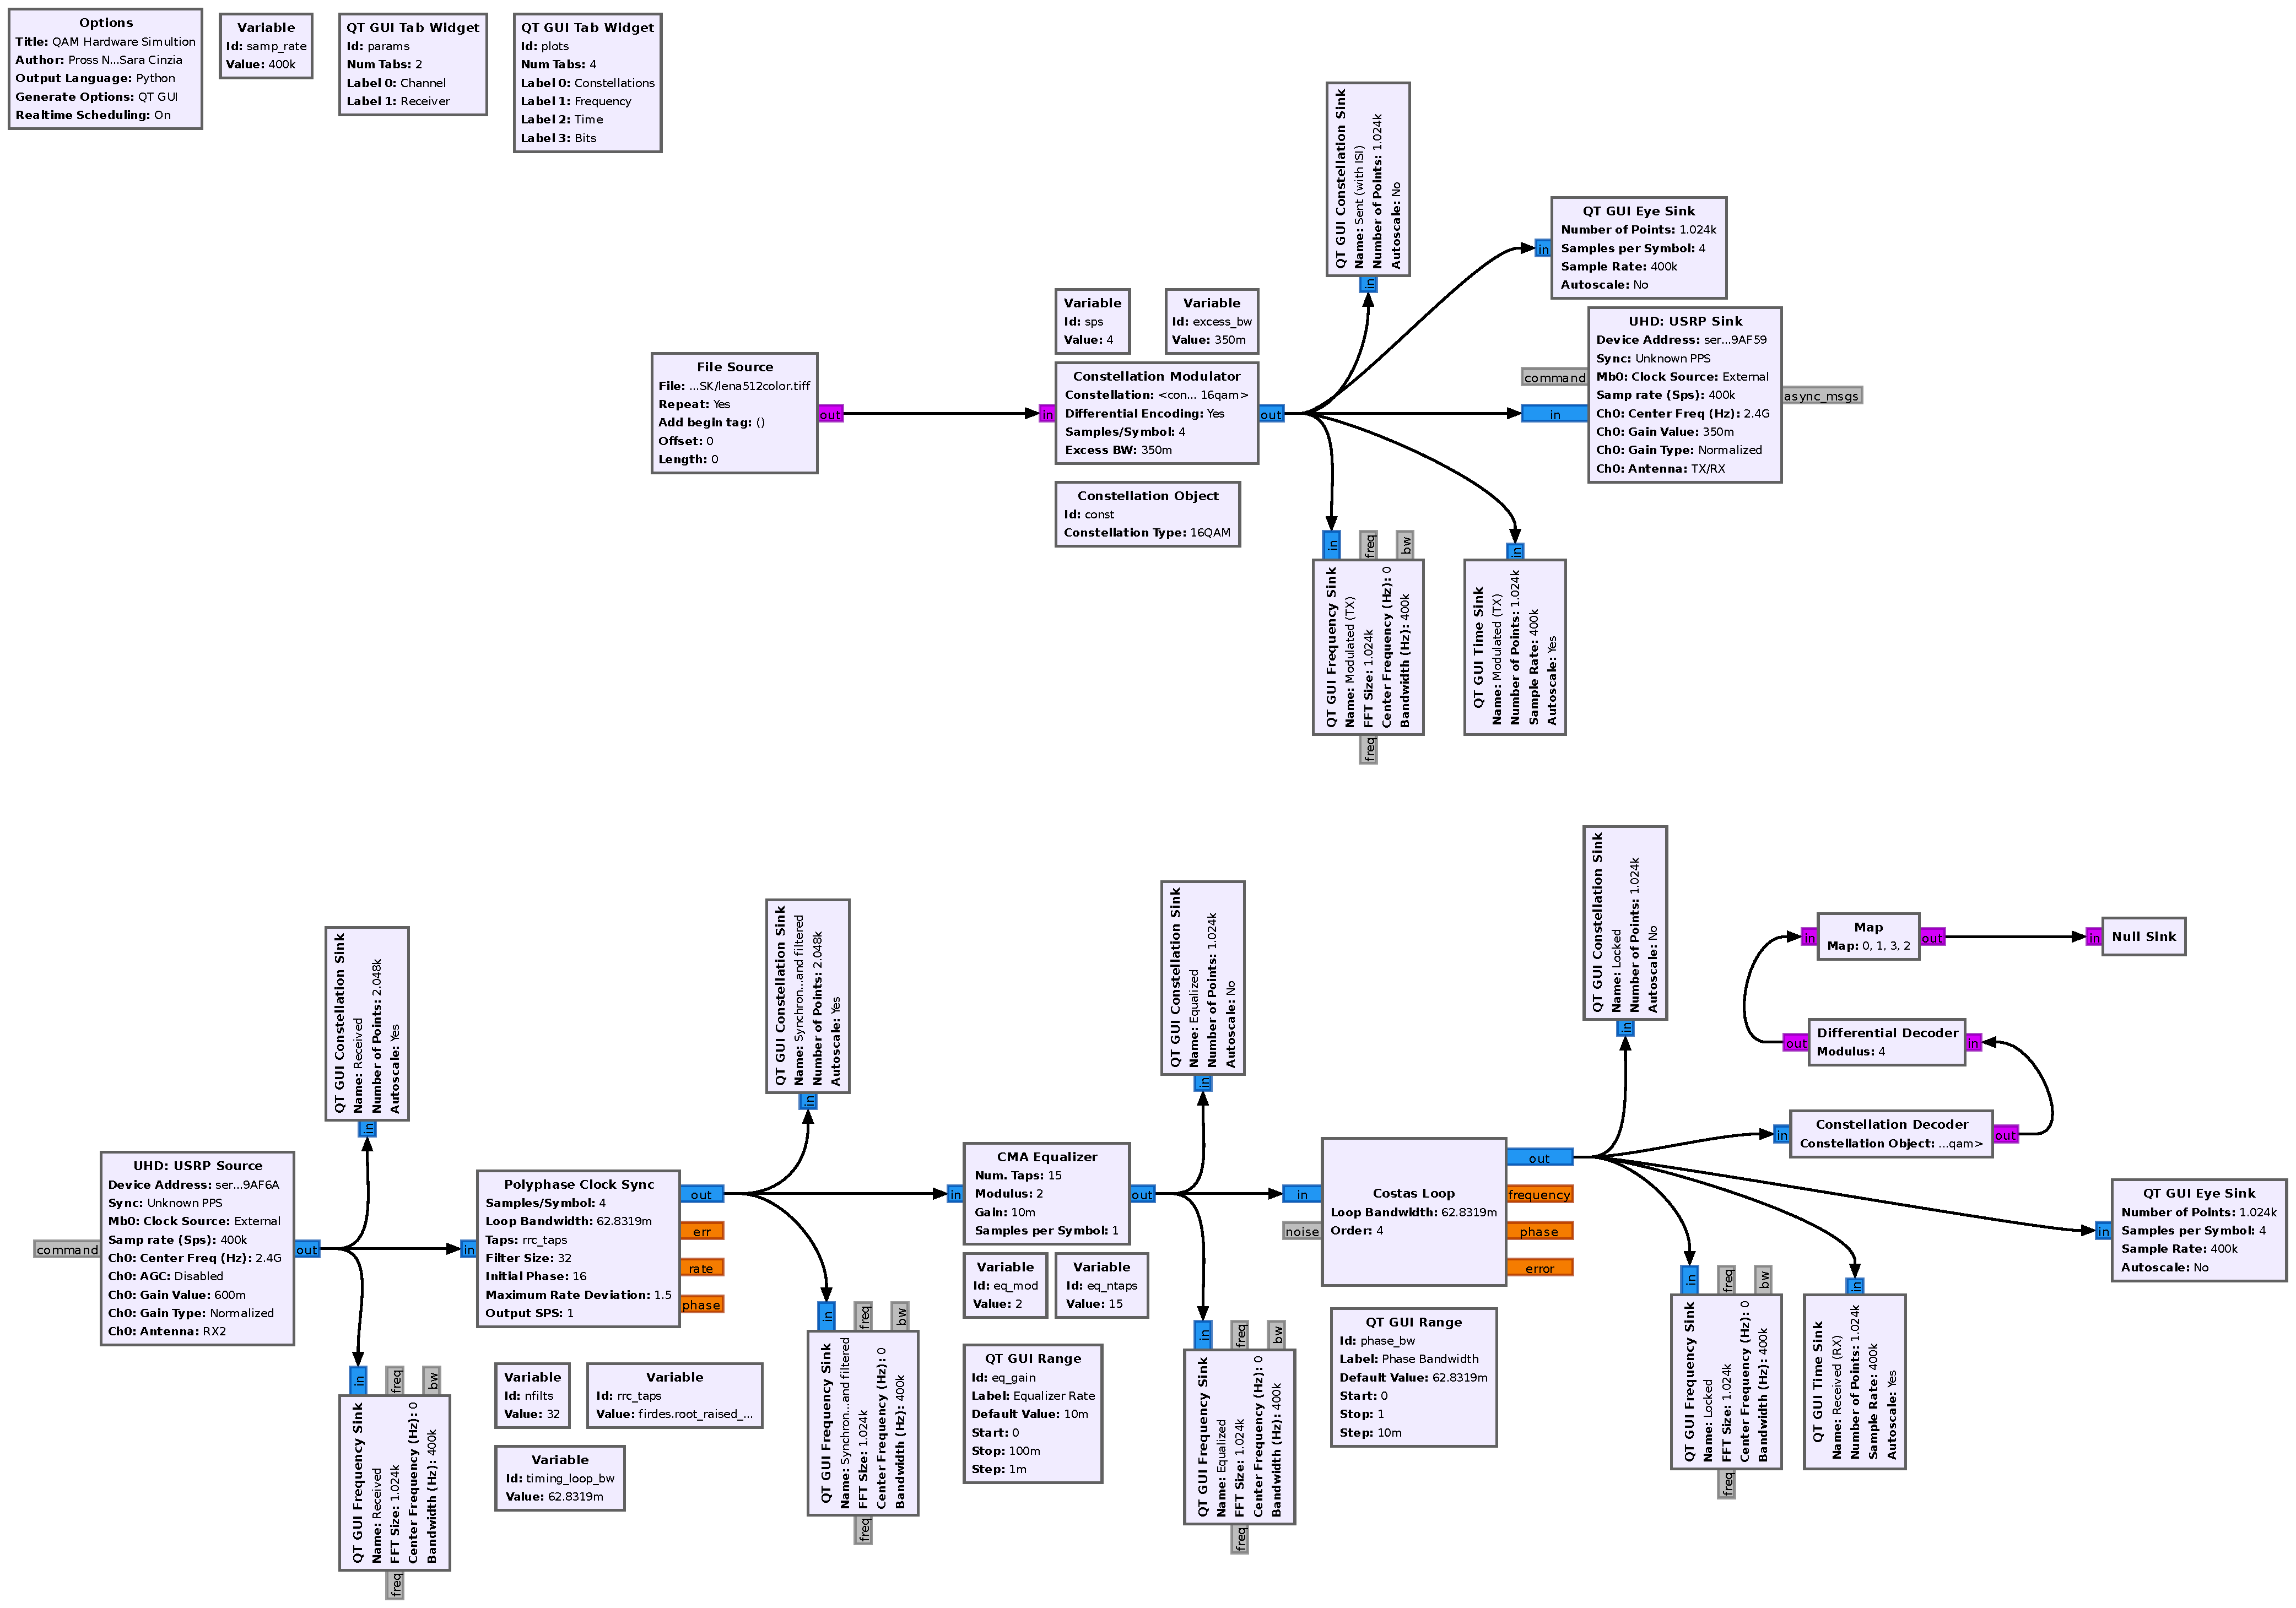
\includegraphics[width=\linewidth]{./figures/pdfs/qam_Hardware_1711.pdf}
	\caption{GNU Radio Blocks Hardware}
	\label{fig:simul16QAM_Hardware_Aufbau}	
\end{figure}

\begin{figure}
	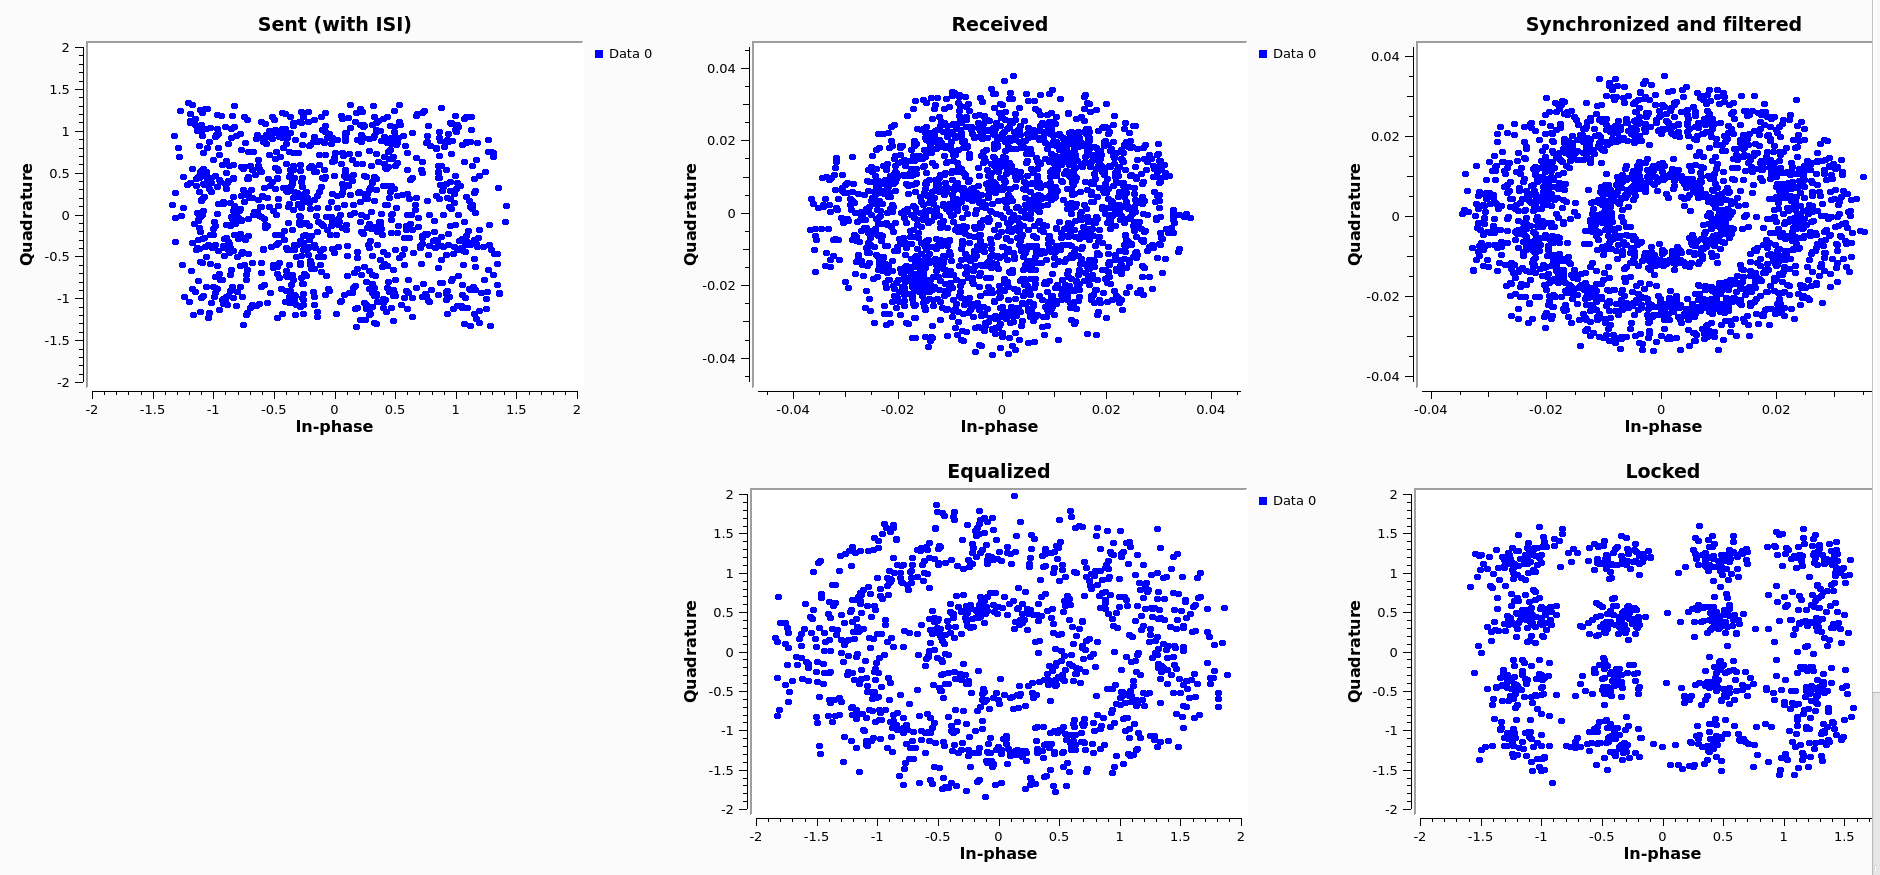
\includegraphics[width=\linewidth]{./figures/screenshots/QAM16_Hardware_1711.png}
	\caption{Hardware results}
	\label{fig:simul16QAM__Hardware}	
\end{figure}

% To Do: Picture of the setup

\begin{table}[]
	%To DO sepzifikationen ampssen / genauer? https://www.ettus.com/wp-content/uploads/2019/01/b200-b210_spec_sheet.pdf
	%https://kb.ettus.com/B200/B210/B200mini/B205mini#FAQ
	\centering
	\caption{USRP B210 specifications}
	\begin{tabular}{ll}
		\toprule
		Dimensions               & \(9.7 \times 15.5 \times 1.5\) cm \\
		Ports                    & 2 TX, 2 RX, Half or Full Duplex     \\
		RF frequencies           & from 70MHz to 6GHz                    \\
		Bandwidth                & 200kHz -- 56MHz                       \\
		External reference input & 10 MHz                                \\
		\bottomrule
	\end{tabular}
\label{tab:USRP B210 specifications}
\end{table}

	% vim: set ts=2 sw=2 noet spell:

\chapter{Conclusions} \label{chp:conclusions}

\section{Results}

The goal to build a functional demonstrator has been only partially achieved, unfortunately not all of the originally planned features could be implemented. A stable wireless link using QPSK modulation that computes the BER was developed. Because of the issue discussed in section \ref{sec:access-code-issue}, the QAM variant cannot compute the empirical BER.

For both modulation schemes samples from multiple different conditions were collected and analyzed, albeit some assessments could only be conducted when QPSK was used.

\section{Future Work}

% raspberry pi

\subsection{Improve BER measurements and simulations}

A missing feature in this work is an automated collection of the BER data, which would allow to more easily to observe and measure the influence of each parameters in the fading channel model.

\subsection{Improvements in the GUI front-end}

In addition to fixing the issue discussed in section \ref{sec:gui-issue-single-threaded}, a very important feature that is currently missing is the ability to change the fading parameters in real time from within the GUI. Dear PyGUI offers many graphical elements that could be used to control the parameters, however a new GR block would need to be created to propagate the updated values into the flow graph.

\subsection{Channel parameters estimation with PSAM}

An interesting continuation of this work could be to regularly interpolate some so called pilot symbols in the modulated data stream. In short, the pilot symbol assisted modulation (PSAM) technique consists of periodically inserting informationless (known) symbols in the data stream, which can then be used to estimate the fading parameters of the communication channel. More details are presented in \cite{Xiaoyi1999} (and its references) from which the illustrations in \figref{fig:psam} were taken.

\begin{figure}
	\centering
	\includegraphics[width = \linewidth]{figures/xiaoyi-psam-figures}
	\caption{
		Illustration of the pilot symbols assisted modulation (PSAM) frame format (left), and PSAM fading interpolation method (right). The PSAM technique allows to compute the fading (denoted in the figure with \(\tilde{z}_n\)) by interpolating measurements of informationless symbols (pilot symbols) over multiple frames. Both figures were taken from \cite{Xiaoyi1999}, which presents an analytical method to compute the BER from the PSAM and multilevel quadrature amplitude modulation (M-QAM) parameters.
		\label{fig:psam}
	}
\end{figure}

\section{Closing words}

\section{Acknowledgments}


We would like to thank everyone who took the time to help us. Specially Michel Nyffenegger, Nicola Ramagnano for their explanations, with the GNU Radio tool,
Marcel Kluser, who has provided the equipment, Prof. Dr. Heinz Mathis for the opportunity and to our friends whose supported us in different ways.





	%% TODO: remove in final version
	\printskelnotes
	\printbibliography

\end{document}
